\documentclass[hidelinks,12pt]{article}
\usepackage[english,brazil]{babel}
\usepackage{hyperref}
\usepackage{graphicx}
\graphicspath{ {images/} }
\linespread{1.3}

\usepackage{geometry}
\geometry{
	a4paper,
	top=30mm,
	left=30mm,
	right=20mm,
	bottom=20mm
}

\usepackage{float}
\usepackage{subcaption}

\usepackage{listings}

\usepackage[titletoc,title]{appendix}
\usepackage{bookmark}
\makeatletter
\renewcommand*\l@section{\@dottedtocline{1}{0em}{1.5em}}
\makeatother
\author{Bruno Yoshikazu Shimada}
\title{\textbf{Desenvolvimento de aplicativo Android paara Micropagamentos}
	}
\date{Novembro 2017}

\begin{document}
\begin{titlepage}
	\centering
	{\Large Universidade de S\~ao Paulo\par}
	{\Large Escola de Artes, Ci\^encias e Humanidades\par}
	\vfill
	{\Large Bruno Yoshikazu Shimada\par}
	\vspace{1cm}
	{\Large\bfseries Desenvolvimento de aplicativo para micropagamentos na plataforma Android\par}
	\vfill
	{\Large S\~ao Paulo\par}
	{\Large 2017\par}
\end{titlepage}
\newpage
\begin{titlepage}
	\centering
	{\Large Bruno Yoshikazu Shimada\par}
	\vspace{2cm}
	{\Large\bfseries Desenvolvimento de aplicativo para micropagamentos na plataforma Android\par}
	\vfill
	\begin{flushright}
		\hspace{7cm}Relat\'orio parcial apresentado \`a Escola de Artes,
	
		\hspace{7cm}Ci\^encias e Humanidades, da Universidade de S\~ao
	
		\hspace{7cm}Paulo, como parte dos requisitos exigidos na
	
		\hspace{7cm}disciplina ACH 2018 - Projeto Supervisionado ou
	
		\hspace{7cm}de Gradua\c{c}\~ao II, para obten\c{c}\~ao do t\'itulo de
	
		\hspace{7cm}Bacharel em Sistemas de Informa\c{c}\~ao.
		\bfseries Orientador: Prof. Dr. Luciano Vieira de Ara\'ujo
	\end{flushright}
	\vspace{2cm}
	{\Large S\~ao Paulo\par}
	{\Large 2017\par}
\end{titlepage}
\newpage
\begin{titlepage}
	\begin{flushleft}
		{\Large Nome: SHIMADA, Bruno Yoshikazu \par}
		{\Large T\'itulo: Desenvolvimento de aplicativo para micropagamentos na plataforma Android \par}
	\end{flushleft}
	\begin{flushright}
		\hspace{7cm}Relat\'orio parcial apresentado \`a Escola de Artes,
		
		\hspace{7cm}Ci\^encias e Humanidades, da Universidade de S\~ao
		
		\hspace{7cm}Paulo, como parte dos requisitos exigidos na
		
		\hspace{7cm}disciplina ACH 2018 - Projeto Supervisionado ou
		
		\hspace{7cm}de Gradua\c{c}\~ao II, para obten\c{c}\~ao do t\'itulo de
		
		\hspace{7cm}Bacharel em Sistemas de Informa\c{c}\~ao.
	\end{flushright}
	\vspace{1cm}
	\begin{flushleft}
		{\Large Aprovado em: \rule{1cm}{1pt}/\rule{1cm}{1pt}/\rule{2cm}{1pt} \par}
	\end{flushleft}
	\vfill
	\centering
		{\Large Banca Examinadora \par}
		\vspace{1cm}
		\begin{flushleft}
			{\Large Prof. Dr:\rule{5cm}{1pt}    Institui\c{c}\~ao:\rule{5cm}{1pt}\par}
			{\Large Julgamento:\rule{4,2cm}{1pt} Assinatura:\rule{5cm}{1pt}\par}
			\vspace{1cm}
			{\Large Prof. Dr:\rule{5cm}{1pt}    Institui\c{c}\~ao:\rule{5cm}{1pt}\par}
			{\Large Julgamento:\rule{4,2cm}{1pt} Assinatura:\rule{5cm}{1pt}\par}
			\vspace{1cm}
			{\Large Prof. Dr:\rule{5cm}{1pt}    Institui\c{c}\~ao:\rule{5cm}{1pt}\par}
			{\Large Julgamento:\rule{4,2cm}{1pt} Assinatura:\rule{5cm}{1pt}\par}
		\end{flushleft}
\end{titlepage}
\newpage
\selectlanguage{brazil}
\section*{\centering{Agradecimentos}}
\pagenumbering{roman}
section
\newpage
\selectlanguage{brazil}
\section*{\centering{Resumo}}

Vivemos em uma \'epoca que a cada dia, novas solu\c{c}\~oes digitais s\~ao lan\c{c}adas para resolver nossos problemas cotidianos de uma maneira simplificada que se incorporam ao nosso cotidiano de uma maneira que ap\'os algum tempo n\~ao conseguimos imaginar como n\'os conseguimos viver sem isso por tanto tempo.

Entre as solu\c{c}\~oes digitais podemos citar por exemplo o ramo econ\^omico e banc\'ario, com desde os b\'asicos aplicativos de bancos para consulta a extratos, pagamentos de boletos, etc, at\'e solu'\c{c}\~oes mais sofisticadas como aplicativos para receber e processar pagamentos por cart\~ao.

Por\'em um problema corriqueiro que temos no dia-a-dia \'e o pagamento de pequenas transa\c{c}\~oes monet\'arias, como tomar um caf\'e na padaria, comprar um chiclete na bomboniere, emprestar uma pequena quantia de dinheiro para um conhecido, entre outras que na maioria das vezes n\~ao passam de 10R\$ e que geram uma perda de tempo de ter que realizar o pagamento com um cart\~ao, digitando a senha pessoal em uma m\'aquina e torcendo para o servi\c{c}o da operadora do cart\~ao estar disponível no momento.

Para resolver esse problema entram em cena os servi\c{c}os de micropagamento, que buscam solucionar o problema de fazer um pagamento ou uma transa\c{c}\~ao de pequeno valor entre duas pessoas, independente de ser pessoa-a-pessoa ou pessoa-a-neg\'ocio, de forma r\'apida, eficaz, segura e descomplicada. O prop\'osito deste trabalho \'e ent\~ao desenvolver um aplicativo Android, SO mais comum entre os usu\'arios de celular no Brasil, que gerencie as transações entre usu\'arios do aplicativo e que fa\c{c}a valer as caracter\'isticas descritas anteriormente.
\newline



\textbf{Palavras Chaves}
\begin{itemize}
	\item Micropagamentos
	\item \textit{Android}
	\item \textit{Fintech}
\end{itemize}
\newpage
\selectlanguage{english}
\begin{abstract}
We live in time that everyday new digital solutions are released to solve our daily problems in a simplified manner, that merges into our days that after some time we are unable to imagine how we lived so much time without it.

Among these digital solutions we can mention for example the economic/banking areas, that has the basic bank app for checking account information, payment of tickets, etc.. To more sophisticated apps that receive and process payments by card.

However a common problem we have in our daily lives is the payment of small monetary transactions, such as having a coffee at a bakery, buying gum from a local store, lending money to an acquaintance, among others that in most times don’t surpass 10 BRL and generate a loss of time for having to make the payment with a card, typing our personal password on a machine and hoping the service of the card operator will be available at the moment.

To solve this problem the micropayments services come into play, seeking to solve the problem of making the payment or transaction of a small amount of money between two persons, regardless of being a person-to-person or person-to-business, in a quick, efficient, safe and uncomplicated way. The purpose of this work is to develop an Android app, the most common OS among mobile users in Brazil, that manage transaction between users of the app and enforce the characteristic described before.
\newline


\textbf{Keywords}
\begin{itemize}
	\item Micropayments
	\item Android
	\item Fintech
\end{itemize}
\end{abstract}
\newpage
\selectlanguage{brazil}
\begingroup
\centering
\listoffigures
\endgroup
\newpage
\selectlanguage{brazil}
\begingroup
\hypersetup{hidelinks}
\tableofcontents
\endgroup
\newpage
\pagenumbering{arabic}
\selectlanguage{brazil}
\section{Introdu\c{c}\~ao}
A defini\c{c}\~ao de micropagamento \'e relativamente simples, se usado uma associa\c{c}\~ao das palavras que a comp\~oem, se infere que se trata de transa\c{c}\~oes cujo valor \'e uma quantia muito pequena. Trazendo para a realidade dele, um micropagamento \'e uma transa\c{c}\~ao online de uma quantia muito pequena de dinheiro (INVESTOPEDIA). Qu\~ao pequeno esse valor \'e, varia entre as diferentes empresas no mercado, o \textit{PayPal}, \textit{e-commerce} que faz a transa\c{c}\~ao de valores digitais entre usu\'arios nas duas pontas, considera um micropagamento qualquer transa\c{c}\~ao cujo valor seja menor do que 10USD (PAYPAL).

A evolu\c{c}\~ao do mercado de  micropagamentos \'e creditada a 3 fatores \textit{(HERNANDEZ - VERME,BENAVIDES;2013)} definidos com base em um relat\'orio de \textit{VASILJEV(2016)} e \textit{BURELLI (2016)}, definem eles como: 
\begin{itemize}
	\item O crescimento da infraestrutura de rede e do e-commerce em geral
	\item O crescimento das redes sociais, jogos online e neg\'ocios de bens digitais
	\item O aparecimento de novas formas de servi\c{c}os de pagamento online
\end{itemize}
Com base nisso podemos ver que as solu\c{c}\~oes atuais para micropagamento surgiram principalmente da necessidade de pagamento de bens para consumo digital como assinaturas de sites, compras de m\'usicas digitais, o melhor exemplo aqui seria o \textit{iTunes} por exemplo.
Dentre as solu\c{c}\~oes que existem atualmente, a \textit{Investopedia} d\'a foco em dois modelos:
\begin{itemize}
	\item A plataforma agindo como carteira digital. Cada usu\'ario cria sua conta na plataforma que ir\'a gerenciar a transa\c{c}\~ao entre dois usu\'arios, a transa\c{c}\~ao \'e efetuada e a plataforma se encarrega de armazenar esse valor, quando a carteira de qualquer uma dessas partes atinge um limite, a quantia total do dinheiro e liberada e transferida para o usu\'ario.
	\item A plataforma agindo com cr\'editos. Cada usu\'ario cria sua conta no plataforma, cada um deles compra/recarrega a quantia desejada que deseja ter como cr\'edito, a cada transa\c{c}\~ao entre duas partes a plataforma se encarrega de atualizar os cr\'editos de ambas as partes.
\end{itemize}
O grande problema na \'area de micropagamentos s\~ao as taxas cobradas pelas operadoras de cart\~ao de cr\'edito, meio que a maioria dos modelos existentes como demonstrado acima usa como forma preferencial de pagamento o cart\~ao cr\'edito, por\'em \'e sabido que para cada transa\c{c}\~ao s\~ao cobradas taxas em cima do valor pago, \'e um caso raro mas podem existir situa\c{c}\~oes que as taxas podem, porque n\~ao, superar o valor da transa\c{c}\~ao, o que para um cliente que seja dono de um neg\'ocio, torna-se algo insustent\'avel.

Uma plataforma de micropagamentos tamb\'em pode se aplicar ao mundo offline como uma forma de currência que substitua o dinheiro padr\~ao em pequenas comunidades.

Imagine por exemplo o ambiente de um condom\'inio privado que ofer\c{c}a servi\c{c}os internos para os condôminos, a forma natural que se imagina que as transa\c{c}\~oes v\~ao ocorrer nesse meio \'e por forma de dinheiro em esp\'ecie, o que levanta alguns riscos para essa popula\c{c}\~ao, sabendo que nessa ambiente circula dinheiro vivo, e que a seguran\c{c}a \'e alguns n\'iveis mais baixa que a comum, alguma pessoa mal intencionada pode pensar em levar vantagem e cometer um assalto contra os prestadores desse servi\c{c}o visando roubar o dinheiro que fica acumulado.

Com o uso de uma plataforma de micropagamentos os condôminos poderiam fazer a carga de uma quantia de dinheiro digital em um aplicativo, os prestadores de servi\c{c}o aceitarem essa forma de pagamento, e a pessoa fazer a transa\c{c}\~ao usando esse dinheiro digital, isso faz com que n\~ao circule dinheiro vivo no ambiente deles, o dinheiro est\'a circulando, por\'em ele est\'a externo ao ambiente, ele n\~ao pode ser acessado de uma maneira f\'isica naquele local o que pode ajudar a inibir pessoas que pensem em roubar o condom\'inio j\'a que n\~ao haveria dinheiro f\'isico no local.

Essa mesma abordagem pode ser aplicada para por exemplo, o restaurante universit\'ario da nossa faculdade. Ao inveś de pagar a carga do cart\~ao com o dinheiro f\'isico, os alunos poderiam fazer isso com um aplicativo, efetuando a carga de cr\'editos com um cart\~ao de cr\'edito por exemplo e pagando na entrada com o seu celular e a funcion\'aria do restaurante com o celular da empresa respons\'avel recebendo os pagamentos.
\newpage
\section{Objetivos}


\subsection{Objetivo Geral}
O objetivo do trabalho foi desenvolver um aplicativo \textit{Android} que conseguisse efetuar micropagamentos entre \textit{smarthphones}.
\newline


\subsection{Objetivos Espec\'ificos}
Os objetivos espec\'ificos do trabalho foram:
\begin{itemize}
	\item Aprendizagem do conceito de micropagamentos
	\item Estudo da bibliografia de artigos de micropagamentos.
	\item Desenvolver a \textit{UI} do aplicativo 
	\item Integrar a interface com base em uma plataforma de servi\c{c}os e infraestrutura existente.
\end{itemize}
\newpage
\section{Revis\~ao Bibliogr\'afica} \label{revisao}
Ao longo do desenvolvimento do aplicativo, em diversos momentos apareceram d\'uvidas que n\~ao conseguiam ser resolvidas por for\c{c}a bruta, como por exemplo, como definir a posi\c{c}\~ao fixa de um bot\~ao em rela\c{c}\~ao a outros no mesmo layout? D\'uvidas desde as mais simples, que surgem principalmente nos momentos iniciais de aprendizado de alguma linguagem ou \textit{framework} novo, at\'e as mais complexas, quando j\'a se tem uma base s\'olida de conhecimento sobre o t\'opico, s\~ao comuns no meio da tecnologia, fato que pode ser comprovado fazendo uma simples busca no \textit{Google}, nas p\'aginas de resultado \'e comum encontrar pessoas com a mesma d\'uvida, em variados f\'oruns, blogs e  sites diversos. O mais interessante nesse ponto \'e a tamb\'em a variedade de abordagens diferentes que s\~ao poss\'iveis de encontrar para uma mesma d\'uvida, fazendo com que tenhamos que filtrar dentre elas a que melhor se aplica ao contexto do nosso problema.

Abaixo est\~ao listadas as fontes consultadas ao longo do trabalho que ajudaram em diversos momentos do desenvolvimento.

Para entendimento do conceito de micropagamentos foram usadas duas fontes principais.

A p\'agina do termo \cite{invest} no site da \textit{Investopedia} que deu uma vis\~ao geral sobre o assunto, enfocando primeiro em um resumo simplificado para depois se aprofundar um pouco mais nele. O interessante desse site \'e que a partir do termo \textit{"micropayment"}, ele busca termos relacionados buscando fazer uma trilha de informa\c{c}\~oes para abranger o assunto.

Outra fonte consultada foi o artigo \textbf{\textit{"Virtual currencies, micropaymentes and the payments systems: a challenge to fiat money and monetary policy?"}} \cite{microp} que discorre n\~ao s\'o sobre o conceito de micropagamentos como tamb\'em aborda o tema das moedas virtuais e relaciona ambos. O artigo foca mais na parte de como os micropagamentos s\~ao mais relevantes no mundo online na compra de itens que eles classificam como microprodutos, fazem uma compara\c{c}\~ao das transa\c{c}\~oes online que envolvem produtos f\'isicos e digitais. Esse artigo considero como o principal usado j\'a que ele aborda de uma maneira mais aprofundada o ambiente que os micropagamentos se inserem.

O artigo \textbf{\textit{"Micropayments: A Viable Business Model?"}} \cite{stanford} apresenta um ponto interessante nas quest\~oes sobre os desafios t\'ecnicos que uma aplica\c{c}\~ao de micropagamentos teria que se preocupar em atender para desenvolver uma aplica\c{c}\~ao segura. Os autores listam 5 pontos que consideram serem desafios que precisam ser vencidos para uma implementa\c{c}\~ao bem-sucedida, seguran\c{c}a, escalabilidade, confiabilidade, interoperabilidade e anonimidade. O interessante desse artigo \'e ele fazer o relacionamento do ecossistema de micropagamentos com os componentes e requisitos desej\'aveis para desenvolvimento de um aplicativo. 

Seguran\c{c}a \'e um requisito necess\'ario para praticamente qualquer aplicativo, por\'em quando tal aplica\c{c}\~ao envolve dinheiro e transa\c{c}\~oes ele se torna um problema de alta prioridade de ser resolvido, ter um aplicativo inseguro que apresente muitas falhas, e entre elas as que sujeitam o aplicativo a sofrer ataques que comprometam as informa\c{c}\~oes e dados de usu\'arios, podem fazer a confian\c{c}a nele cair, o que reduz a base de usu\'arios. Os autores nesse item que durante o desenvolvimento \'e preciso tomar aten\c{c}\~ao com autentica\c{c}\~ao, autoriza\c{c}\~ao, integridade de informa\c{c}\~ao e confidencialidade.

Arquitetar o sitema de uma maneira que permita que ela seja escal\'avel \'e um requisito necess\'ario para poder lidar com um pontencial aumento do número de acessos a aplica\c{c}\~ao. O desenho da solu\c{c}\~ao deve ser de tal forma que seja poss\'ivel acoplar mais servidores a medida que foram necess\'arios para poder lidar com o tr\'afego de informa\c{c}\~oes.

É levantado tamb\'em a quest\~ao de interoperabilidade, permitir que diferentes aplica\c{c}\~oes de micropagamentos conversem entre si, este talvez seja o ponto de maior dificuldade de se atingir. Aplica\c{c}\~oes diferentes possuem diferentes meios de tratar a informa\c{c}\~ao que chega, sai, e processada nele.


A quest\~ao da anonimidade \'e tratado como um ponto complicado de se definir, at\'e que ponto a anonimidade deve existir a a partir de que ponto \'e necess\'ario saber a identididade dos usu\'arios, quanto um usu\'ario pode e deve saber do outro, quest\~oes que valem para os dois atores envolvidos em um micropagamento. O artigo n\~ao levanta nennhuma resposta definitiva sobre o assunto, ele apresenta bons argumentos a favor e contra a quantidade de anonimidade no sistema.

Um dos exemplos \'e explorado \'e o registro de hist\'orico de transa\c{c}\~oes, para um usu\'ario que faz o pagamento \'e uma informa\c{c}\~ao útil de ser acessada, mas que precisa de uma pequena fra\c{c}\~ao de depriva\c{c}\~ao de anonimidade. Mas ao mesmo tempo \'e informa\c{c}\~ao que pode ser usada por terceiros para descobrir padr\~oes de consumo e o que foi consumido, e que pode ser usado contra o usu\'ario. Um \textit{e-commerce} por exemplo, com base nessas informa\c{c}\~oes pode manipular os pre\c{c}os e anúncios que tem potencial de ser interesse de tal usu\'ario.
% link do training para android

No come\c{c}o do projeto meu conhecimento de programa\c{c}\~ao para \textit{Android} era nulo, durante a prepara\c{c}\~ao da m\'aquina encontrei no mesmo site que disponibiliza a \textit{IDE} para desenvolvimento, uma sub-se\c{c}\~ao intitulada \textit{Training}, debaixo da se\c{c}\~ao \textit{Develop} \cite{anddev}. Nela encontrei uma s\'erie de li\c{c}\~oes b\'asicas para quem est\'a come\c{c}ando a desenvolver para \textit{Android}. Foi \'util para ter uma no\c{c}\~ao b\'asica de onde come\c{c}ar e os termos espec\'ificos usados.

Ap\'os a cria\c{c}\~ao de um aplicativo \textit{Hello World} b\'asico seguindo o guia \cite{androidhw} do site da \textit{Android}, fui atr\'as de mais algum material para criar um aplicativo e aprofundar um pouco mais o conhecimento na plataforma. O livro \cite{andppe} utilizado nesse momento foi \textbf{\textit{"Android 5 Programming by Example"}}, o livro \cite{andppe} se aprofunda um pouco mais nos exerc\'icios ajudando e servindo de guia para criar um aplicativo mais robusto do que o visto no guia do site da \textit{Android}. O livro \cite{andppe} foi usado de guia no segundo passo do projeto onde criei um aplicativo \textit{mock} que simulava localmente uma transa\c{c}\~ao nos moldes de um micropagamento de um aparelho para um servidor, para testar os conhecimentos e novas t\'ecnincas adquiridas. Apesar do livro \cite{andppe} focar mais na vers\~ao \textit{Lollipop}, lan\c{c}ada em 2015 mesmo ano da publica\c{c}\~ao do livro, grande parte dos componentes n\~ao mudou muito para a vers\~ao mais atual.


Durante a elabora\c{c}\~ao do rascunho das interfaces do aplicativo uma p\'agina \cite{material} que foi muita usada como fonte de consulta e guia \'e a \textit{Material Design}. Nela foi poss\'ivel encontrar orienta\c{c}\~oes e guias de como desenhar a interface para se encaixar no padr\~ao do \textit{Material Design}. A seguir s\~ao descritas as ferramentas e guias dispon\'iveis que se destacam pelo seu uso e importância no projeto.

A p\'agina \textbf{\textit{Material Icons}} \cite{materialicon} \'e uma esp\'ecie de repos\'itorio da \textit{Google} com v\'arios \'icones dispon\'iveis para uso. Todos s\~ao liberados para uso sobre a licen\c{c}a \textit{Apache License Version 2.0}. Os \'icones s\~ao desenhados de maneira simples e de f\'acil interpreta\c{c}\~ao, o design deles \'e de uma maneira que quando se olha para o \'icone \'e f\'acil deduzir qual seu significado. Por exemplo o \'icone da figura \ref{icon_pay} que foi usado para simbolizar a a\c{c}\~ao de pagamento:
	% (inserir \'icone do pagamento)
	\begin{figure}[h]
		\centering
		
\includegraphics{pay_action_white}
		\caption{\'Icone usado para simbolizar a a\c{c}\~ao de pagamento}
		\label{icon_pay}
	\end{figure}

	Al\'em da p\'agina com o rep\'ositorio dos \'icones, o design e o conceito dos itens \'e explicado no artigo \textbf{\textit{Style - Icons}} \cite{materialiconguide}
	
A p\'agina \textbf{\textit{Material Colors}} \cite{materialcolors} possui uma ferramenta \cite{materialcolorpallete} que ajuda na escolha da paleta de cores que v\~ao compor o aplicativo, ele oferece tamb\'em um guia visual de como ficam as cores nas interfaces do sistema. Outro artigo relacionado \'e \textbf{\textit{Style - Colors}} \cite{materialcolors} onde \'e explicado as boas pr\'aticas e guias para selecionar as cores dos componentes da interface do aplicativo.

\newpage
\section{Metodologia}

Para o projeto eram necess\'arios conhecimentos em dois t\'opicos, micropagamentos e \textit{Android}. Inicialmente foi feito um estudo da bibliografia de micropagamentos, descrita no cap\'itulo \ref{revisao}, para entender melhor o conceito dele como um todo, suas caracter\'isticas, limites, o panorama atual e o mercado. Tendo aprendido esse conceito foi feito um estudo buscando aprender os conceitos da programa\c{c}\~ao para \textit{Android}, posteriormente foram desenvolvidos alguns aplicativos de teste para aplicar o conhecimento adquirido.

Adquiridos os fundamentos necess\'arios sobre os dois assuntos dei andamento no trabalho para definir o escopo dele, foram definidas quantas e quais interfaces seriam necess\'arias para atingir o objetivo proposto, desenvolver a interface de um aplicativo \textit{Android} com base numa plataforma de servi\c{c}os existentes buscando fazer a mesma ser simples, no sentido de ter uma f\'acil utiliza\c{c}\~ao, buscando obedecer e seguir os guias definidos pelo \textit{Android} como boas pr\'aticas e que atendem e se adequam a filosofia do \textit{Material Design}. Foram avaliados nesse momento as estruturas e componentes que seriam usados, como por exemplo bot\~oes, layouts, esquema de cores, etc.

Definida as interfaces passei a avaliar a estrutura de servi\c{c}os com as quais as interfaces seriam integradas, foi o momento de aprender como funcionava a plataforma, como ela se comunicava internamente entre suas classes, quais eram as entradas e sa\'idas de cada momento. Com isso foi refinado a etapa anterior de defini\c{c}\~ao das interfaces para se adequar a plataforma, foram revistas as interfaces imaginadas,adicionando e retirando alguns componentes visuais, e criadas novas interfaces.

Com o escopo definido foi feito uma avalia\c{c}\~ao de esfor\c{c}o para definir o cronograma que seria seguido e dado in\'icio ao desenvolvimento das interfaces do aplicativo.

Para o desenvolvimento das interfaces do aplicativo, e controle das a\c{c}\~oes foram utilizadas duas linguagens no trabalho:
\begin{itemize}
	\item \textbf{\textit{XML}}: todas as interfaces do \textit{Android} s\~ao escritas usando a linguagem de marca\c{c}\~ao \textit{XML}, o \textit{Android} usa um conjunto de elementos e atributos pr\'oprios na marca\c{c}\~ao como por exemplo o elemento \textit{\textless{RelativeLayout}\textgreater} e o atributo \textit{android:layout\_width}. \textit{XML} tamb\'em usado para definir \textit{Strings}, o tema base, e qualquer outro elemento visual que possa ser reaproveitado, como por exemplo um \textit{layout} customizado para um bot\~ao. Tamb\'em \'e usado para definir o manifesto do aplicativo, onde s\~ao declaradas configur\~a\c{c}\~oes espec\'ificas do aplicativo, como por exemplo permiss\~ao para uso de \textit{bluetooth}, \textit{internet}, etc.
	\item \textbf{\textit{Java}}: A parte do \textit{back-end} que controla a aplica\c{c}\~ao \'e toda codificada em \textit{Java}. O \textit{Android} usa \textit{Java} para por exemplo codificar um \textit{listener} que capta quando o usu\'ario clica em algum bot\~ao por exemplo, para fazer a troca de interfaces, controle de sess\~ao, carregar \textit{Strings} dinâmicas na interface, tratamento de erros e exce\c{c}\~oes, etc.
\end{itemize}

Quanto a \textit{hardware} foram usados um \textit{notebook} pr\'oprio rodando um SO \textit{Debian}, e dois aparelhos celulares pr\'oprios com SO \textit{Android} para simular o comportamento de dois usu\'arios. Devido a diferen\c{c}a de SO de ambos, foi interessante observar como a interface se comportava em cada um deles. A t\'itulo de curiosidade seguem as especifica\c{c}\~oes:
\begin{itemize}
	\item \textit{Notebook}
	\begin{itemize}
		\item SO: \textit{Ubuntu 16.04 LTS - 64-bit}
		\item Mem\'oria RAM: 8GB
		\item Processador: \textit{Intel\textregistered Core\textsuperscript{TM} i7-5500U CPU @ 2.40GHz x 4}
		\item Processador gr\'afico: \textit{Intel\textregistered HD Graphics 5500 (Broadwell GT2)}
	\end{itemize}
	\item Celular \textit{Motorola Moto G} 3\textsuperscript{\underline{a}} Gera\c{c}\~ao
	\begin{itemize}
		\item SO: \textit{Android 5.1 Lollipop}
		\item Mem\'oria RAM: 1GB
		\item Processador: \textit{Qualcomm Snapdragon 410}
	\end{itemize}
	\item Celular \textit{Samsung S3 Mini}
	\begin{itemize}
		\item SO: \textit{Android 4.1 Jellybean}
		\item Mem\'oria RAM: 1GB
		\item Processador: \textit{Dual-core, 1000 MHz}
	\end{itemize}
\end{itemize}
\newpage
\section{Resultados}

\subsection{Desenvolvimento das interfaces} \label{learn}
% start new block
Foram definidas inicialmente para o trabalho o desenho de 4 interfaces, \textit{login}, uma tela principal com as a\c{c}\~oes permitidas ao usu\'ario, a tela de efetuar o micropagamento e a tela de confirma\c{c}\~ao do pagamento, ap\'os estudo da estrutra da plataforma de servi\c{c}os e revis\~ao das interfaces, o número de interfaces que seriam necess\'arias ficou em 13. Para cada uma delas ser\'a descrita o que foi feito e os componentes usados.

Para o desenvolvimento das interfaces foi levantado duas abordagens diferentes, o uso de \textit{RelativeLayout} ou o uso do \textit{ConstraintLayout}, ambas alternativas foram testadas para mensurar as possibilidades e dificuldades que cada uma apresentava, por fim foi escolhido seguir o desenvolvimento usando o primeiro. A vantagem no uso do \textit{Relative Layout} \'e poder declarar a posi\c{c}\~ao dos componentes de acordo com seus parentes ou seus irm\~aos, ele d\'a um maior controle sobre os itens no \textit{layout}. Por exemplo, temos uma \textit{view} que define uma \'area retangular na interface, e dentro dessa \'area precisam estar 3 outros componentes, vamos dizer bot\~oes, e esses 3 componentes precisam estar alinhados à direita da \'area. Com o \textit{RelativeLayout} declaramos a \'area, o primeiro bot\~ao alinhado a direita da \'area, e cada um dos bot\~oes subsequentes um abaixo do outro, com a \textit{ConstraintLayout} o mesmo processo precisa que algumas propriedades a mais sejam usadas para obter o mesmo resultado.

A primeira interface a ser feita foi a de cadastro de us\'ario (referencia a imagem). No fluxo de execu\c{c}\~ao normal, essa interface \'e a primeira, por\'em ela deve ocorrer apenas uma vez no momento que o usu\'ario vai se cadastrar, se o usu\'ario j\'a fez o cadastro essa tela n\~ao volta a ser exibida sendo exibida no seu lugar a interface de \textit{login} (referencia a imagem).

Para a interface de cadastro (referencia a imagem) foram necess\'arios avaliar e estudar a implementa\c{c}\~ao de três tipos de componentes: \textit{EditText}, \textit{Button} e \textit{ImageView}, os três componentes n\~ao apresentaram grande dificuldade em assimilar o comportamento e o que deveria ser feito para aplicar na interface.

O componente \textit{EditText}, simplificadamente, permite que o usu\'ario insira caract\'eres na interface para serem interpretados pela aplica\c{c}\~ao. Na interface eram necess\'arios que o usu\'ario entrasse com duas \textit{strings}, uma para que ele definisse qual o nome de usu\'ario e outra para a senha. A de entrada do nome de usu\'ario foi mais direta a aplica\c{c}\~ao, a entrada de \textit{strings} \'e um componente padr\~ao que n\~ao precisou de muita configura\c{c}\~ao, a de senha era necess\'ario aplicar uma m\'ascara que ocultasse os caract\'eres a medida que eles fossem digitados, por quest\~ao de seguran\c{c}a e privacidade, o efeito desejado foi facilmente obtido apenas atribuindo o valor \textit{textPassword} na propriedade \textit{InputType}, essa propriedade \'e a que controla, nesse caso, se deve ser aplicado uma m\'ascara de senha, ou como ser\'a visto mais a frente, se o teclado de entrada deve exibir apenas n\'umeros ou n\'umeros e letras.

O componente \textit{Button} e o \textit{ImageView} exigiram menos customiza\c{c}\~ao para serem aplicados, o bot\~ao exigiu apenas que fossem definidos as cores de fundo e de texto que s\~ao exibidos nele, a imagem apenas que fosse indicado qual o caminho e identificador da imagem. Um ponto a ressaltar que encontrei dificuldade foi no posicionamento correto da imagem no \textit{layout}, foi preciso voltar a documenta\c{c}\~ao do \textit{Android} para entender a hierarquia de \textit{views} \cite{viewslay} e entender onde a imagem deveria ser posicionada para apresentar o comportamento esperado.

Em seguida foi feita a interface de \textit{login} (referencia para a imagem), j\'a que ela tamb\'em \'e uma das interfaces de entrada do aplicativo, como explicado acima essa tela ap\'os o usu\'ario se cadastras \'e a primeira que vai ser carregada, ela n\~ao precisou que fosse implementado nenhum componente novo, os usados aqui foram os mesmo da interface de cadastro descritos acima. Uma diferen\c{c}a entre elas \'e que como a única entrada de texto necess\'ario \'e a senha do usu\'ario n\~ao foram usados \textit{TextView} para indicar o que \'e para ser iserido no campo, em seu lugar foi usado a propriedade \textit{hint} que, como o nome indica, exibe uma dica para o usu\'ario do que deve ser colocado no campo, e desaparece quando o usu\'ario clica nele.

% end new block
Um dos objetivos espec\'ificos para esse projeto era aprender desenvolvimento para a plataforma \textit{Android}. At\'e o in\'icio do projeto eu nunca havia tido contato com o desenvolvimento para \textit{Android}, ent\~ao o primeiro passo foi ir atr\'as de material sobre o mesmo, o ponto inicial para isso assumi que seria o site oficial da plataforma, isso por experiências passadas de estudo onde a p\'agina de alguma linguagem, \textit{framework}, etc, em grande partes dos casos possuia uma boa documenta\c{c}\~ao sobre a mesma. A p\'agina da plataforma do \textit{Android} felizmente seguia essa linha, e na mesma encontrei as informa\c{c}\~oes necess\'arias para dar in\'icio no aprendizado.

Ap\'os a configura\c{c}\~ao do ambiente, instalando \textit{Java} e a \textit{IDE} apenas, segui o tutorial \cite{androidhw} que explica como criar um aplicativo b\'asico (imagem \ref{hw}) para testar as configura\c{c}\~oes locais. O resultado \'e um aplicativo com duas \textit{Activities} (interfaces), a primeira (imagem \ref*{hw_message}) possui uma \textit{EditText} para escrever uma mensagem e um bot\~ao que chama a pr\'oxima \textit{Activity}, a segunda (imagem \ref*{hw_result}) \textit{Activity} apenas exibe a mensagem escrita.
%inserir as imagens da primeira e segunda tela
\begin{figure}[H]
	\begin{subfigure}{0.5\textwidth}
		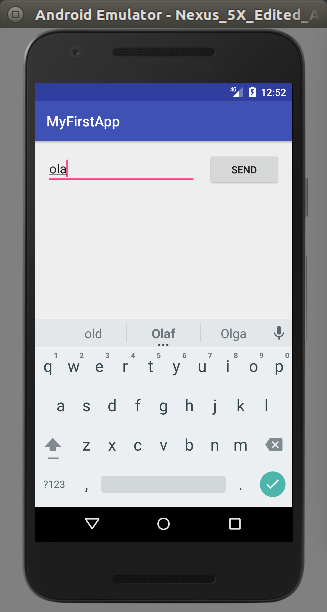
\includegraphics[scale=0.5]{hw_message} 
		\caption{Interface do aplicativo que\\\hspace{\textwidth}recebe um texto e envia para a \\\hspace{\textwidth}pr\'oxima interface}
		\label{hw_message}
	\end{subfigure}
	\begin{subfigure}{0.5\textwidth}
		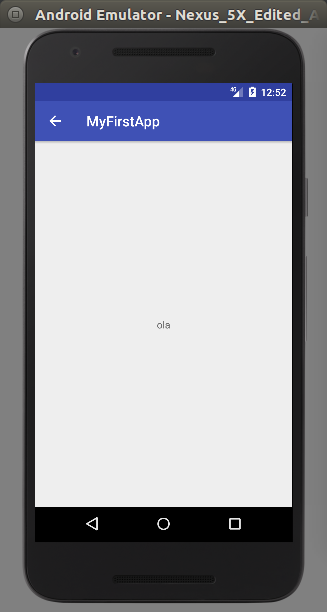
\includegraphics[scale=0.5]{hw_result}
		\caption{Interface que exibe a mensagem\\\hspace{\textwidth}da \textit{Activity} anterior\\\hspace{\textwidth}}
		\label{hw_result}
	\end{subfigure}
	\caption{Interfaces do aplicativo do tutorial}
	\label{hw}
\end{figure}

Apesar de ser um exemplo um tanto trivial, ele engloba alguns aspectos importantes do \textit{Android}:
\begin{itemize}
	\item Cria\c{c}\~ao de interface
	\item Cria\c{c}\~ao de componentes para a interface
	\item Uso de \textit{intents} para trafego de dados entre as interfaces
	\item Procurar, extrair e exibir textos nas interfaces a partir do ID
\end{itemize}

Ap\'os o contato inicial com a plataforma e o desenvolvimento do aplicativo acima, fui em uma busca de mais material e comecei a ler o livro \textbf{"\textit{{Android}} 5 Programming by Example"} \cite{andppe}. Com o conhecimento sobre micropagamentos, o livro citado e os guias, todos indicados na se\c{c}\~ao \ref{revisao}, iniciei o desenvolvimento de um aplicativo que simulasse um micropagamento, o aplicativo era totalmente \textit{offline} e apenas fazia um \textit{mock} de servi\c{c}o de transa\c{c}\~oes.

Para o aplicativo tentei imaginar qual o m\'inimo de interfaces que precisaria para simular o uso do aplicativo por um usu\'ario que queria executar uma transa\c{c}\~ao, e cheguei as seguintes interfaces:
\begin{enumerate}
	\item \label{int:login}Interface de acesso, com espa\c{c}o para o usu\'ario colocar o seu login, a senha, um bot\~ao de confirma\c{c}\~ao e o logo do aplicativo
	\item \label{int:main_list}Interface principal do aplicativo com as a\c{c}\~oes que o usu\'ario pode fazer mapeadas em bot\~oes
	\item \label{int:pay}Interface de pagamento onde o usu\'ario preenche quem \'e o destinat\'ario, o valor, a data e confirma
	\item \label{int:confirm}Interface de confirma\c{c}\~ao da transa\c{c}\~ao
\end{enumerate}
Essas interfaces foram decididas como as principais para desenvolver e testar o conceito de micropagamento em uma escala absurdamente menor, em um ambiente controlado apenas para validar id\'eias e testar conceitos novos no desenvolvimento de interfaces para \textit{Android}.

A interface de \textit{login} (item \ref{int:login}) foi a primeira a ser desenvolvida, \'e a interface mais simples do aplicativo. Os pontos novos do aprendizado nessa interface foram inserir uma imagem na tela e colocar um campo texto do tipo senha, em que os caract\'eres aparecem como asterisco a medida que s\~ao digitados. A interface por fim est\'a ilustrada na imagem \ref{int:login_img}.

A interface principal (item \ref{int:main_list}) do aplicatvo foi a segunda, o ponto novo aplicado nessa interface foi a inclus\~ao de \'icones dentro de um \textit{Button}. A interface est\'a ilustrada na imagem \ref{int:main}.
\begin{figure}[H]
	\begin{subfigure}{0.5\textwidth}
		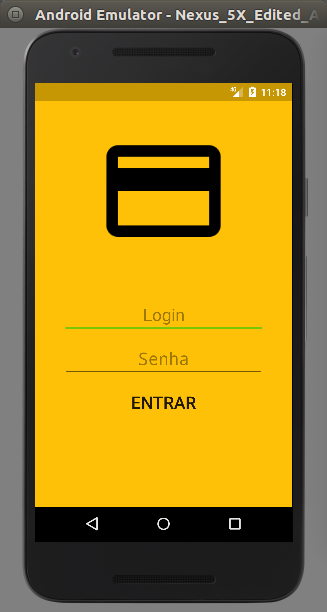
\includegraphics[scale=0.5]{int:login}
		\caption{Interface de \textit{login}\\\hspace{\textwidth}\\\hspace{\textwidth}}
		\label{int:login_img}
	\end{subfigure}
	\begin{subfigure}{0.5\textwidth}
		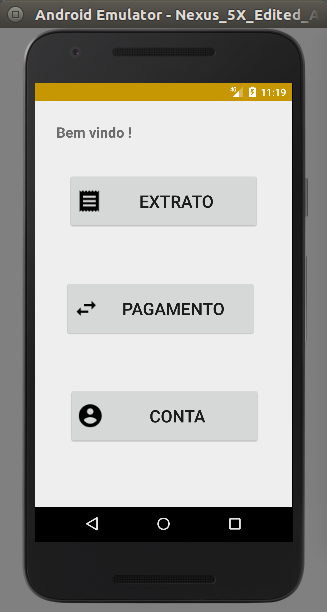
\includegraphics[scale=0.5]{int:main}
		\caption{Interface principal do aplicativo\\\hspace{\textwidth}com as a\c{c}\~oes permitidas ao\\\hspace{\textwidth}usu\'ario mapeadas como bot\~oes}
		\label{int:main}
	\end{subfigure}
	\caption{Interfaces do aplicativo \textit{mock}}
	\label{loginmain}
\end{figure}

A interface de pagamentos (item \ref{int:pay}) \'e a que considerei a mais interessante de se fazer, ela possui dois elementos visuais que demandaram grande esfor\c{c}o para entender o funcionamento e a aplica\c{c}\~ao, um deles \'e um calend\'ario para selecionar datas e o outro \'e uma barra deslizante que de acordo com a posi\c{c}\~ao define qual o valor da transa\c{c}\~ao.

Dentre os dois o que gerou maior dificuldade para ser feito foi o calend\'ario, o \textit{Android} fornece um DatePicker padr\~ao, por\'em ele n\~ao se adequava a implementa\c{c}\~ao desejada, o que busquei fazer para o funcionamento dele era que ao clicar em um campo de entrada de texto comum, abrisse um calend\'ario para que o usu\'ario escolhesse a data e ao finalizar fechasse o calend\'aro novamente.

Para atingir esse efeito foi necess\'ario criar um Fragment que implementasse o DatePicker padr\~ao do \textit{Android}, foi sobreescrito o m\'etodo de onCreate para que ao criar o Fragment retornasse um DatePicker com a data atual. A implementa\c{c}\~ao do Fragment pode ser vista na \textit{listing} \ref{datepicker}.
\newpage
\begin{lstlisting}[language=Java, caption=\textit{Fragment} do calend\'ario, captionpos=b, breaklines=true, label=datepicker]
public class DatePickerFragment extends DialogFragment implements DatePickerDialog.OnDateSetListener{
	@Override
	public Dialog onCreateDialog(Bundle savedInstanceState) {
		final Calendar calendar = Calendar.getInstance();
		int year = calendar.get(Calendar.YEAR);
		int month = calendar.get(Calendar.MONTH);
		int day = calendar.get(Calendar.DAY_OF_MONTH);
		return new DatePickerDialog(getActivity(), (TransactionActivity)getActivity(), year,month,day);
	}
\end{lstlisting}
No c\'odigo de controle da \textit{Activity} foi preciso adicionar um \textit{listener} no campo texto que fica aguardando um 'clique', quando \'e clicado, chama uma fun\c{c}\~ao que instancia o \textit{Fragment} e exibe na interface, ainda nesse controle foi criada uma fun\c{c}\~ao que atribui ao campo do calend\'ario a data selecionada, essa fun\c{c}\~ao \'e sobreescrita de uma definida na mesma classe do \textit{Fragment} do \textit{DatePicker} (ver \textit{listing} \ref{datepicker}).

Um exemplo de como o \textit{Fragment} \'e carregado e renderizado na tela pode ser visto na imagem \ref{main_calendar}. A imagem \ref{int:main_nocal} mostra a interface ao ser carregada, nesse momento o \textit{listener} est\'a aguardando um 'clique' na \'area de texto ao lado de \textbf{Escolha uma data} para carregar o calendário. A imagem \ref{int:main_cal} mostra o \textit{Fragment} carregado na interface.
\begin{figure}[H]
	\begin{subfigure}{0.5\textwidth}
		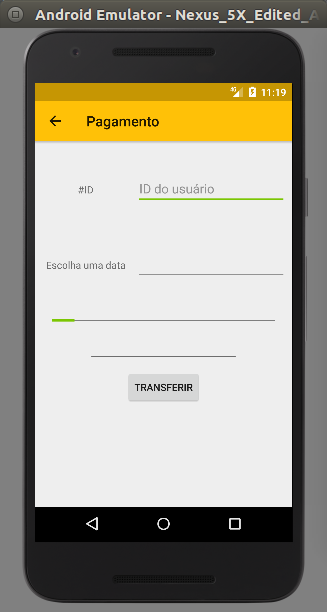
\includegraphics[scale=0.5]{int:main_nocal}
		\caption{\textit{DatePicker} n\~ao\\\hspace{\textwidth}selecionado}
		\label{int:main_nocal}
	\end{subfigure}
	\begin{subfigure}{0.5\textwidth}
		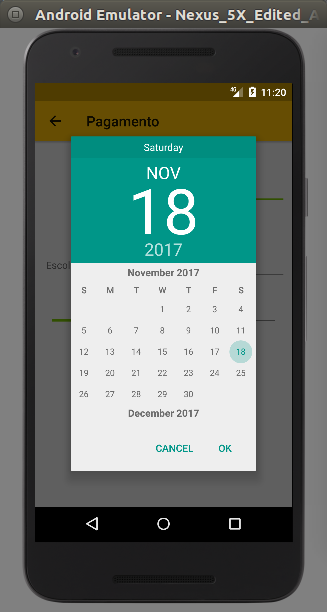
\includegraphics[scale=0.5]{int:main_cal}
		\caption{\textit{Fragment} do \textit{DatePicker} \\\hspace{\textwidth}carregado}
		\label{int:main_cal}
	\end{subfigure}
	\caption{Exemplo de uso do \textit{Fragment} do \textit{DatePicker}}
	\label{main_calendar}
\end{figure}

Para o outro componente, a barra deslizante chamada de \textit{SeekBar}, a implementa\c{c}\~ao exigiu menos codifica\c{c}\~ao, n\~ao foi necess\'ario criar classes adicionais como feito no \textit{DatePicker} (\textit{listing} \ref{datepicker}), j\'a que o componente padr\~ao atendia as necessidades da interface, o que precisou ser codificado foi implementar um \textit{listener} na barra para detectar movimentos nela e sobrepor 3 m\'etodos padr\~oes que definem as a\c{c}\~oes de in\'icio, fim e mudan\c{c}a de status. A de \'inicio n\~ao faz nada, apenas \'e instanciada para definir a barra, a de mudan\c{c}a de status pega o valor de onde a barra parou e atribui \`a uma var\'iavel e a final \'e encarregada de atualizar o campo texto com o valor atual selecionado. A implementa\c{c}\~ao pode ser vista na \textit{listing} \ref{seekbar}.
\newpage
\begin{lstlisting}[language=Java, caption=\textit{SeekBar} do valor, captionpos=b, breaklines=true, label=seekbar]
SeekBar seekbar = (SeekBar) findViewById(R.id.seekBar);
seekbar.setOnSeekBarChangeListener(new SeekBar.OnSeekBarChangeListener(){
	int actual_value = 0;
	@Override
	public void onProgressChanged(SeekBar seekBar, int new_value, boolean b) {
		actual_value = new_value;
	}
	@Override
	public void onStartTrackingTouch(SeekBar seekBar) {
	}
	@Override
	public void onStopTrackingTouch(SeekBar seekBar) {
		TextView transferValue = (TextView) findViewById(R.id.rvalueTransfer);
		transferValue.setText(Integer.toString(actual_value);
	}
});
\end{lstlisting}

A última interface, \'e a de confirma\c{c}\~ao do pagamento (item \ref{int:confirm}), \'e uma tela simples que apenas carrega as informa\c{c}\~oes inseridas na interface anterior (ver imagem \ref{int:main_nocal}) para confirma\c{c}\~ao e execu\c{c}\~ao, lembrando que execu\c{c}\~ao no contexto atual \'e uma simula\c{c}\~ao, do pagamento. Essa interface n\~ao teve nenhum desenvolvimento expressivo j\'a que ela usa elementos, nesse ponto do aprendizado, b\'asicos, como campos textos carregando informa\c{c}\~oes vindos da leitura da \textit{Intent} que transportou os dados de uma \textit{Activity} para outra.

\begin{figure}[H]
	\begin{subfigure}{0.5\textwidth}
		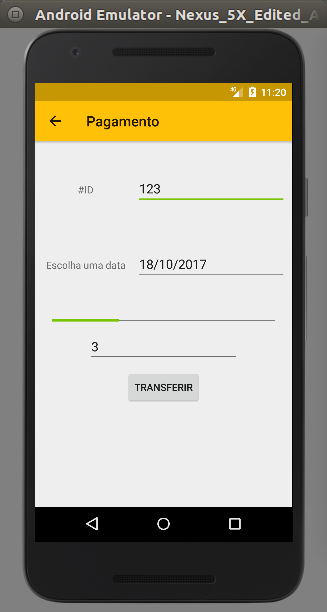
\includegraphics[scale=0.5]{int:pay}
		\caption{Interface com todas as\\\hspace{\textwidth}informa\c{c}\~oes preenchidas}
		\label{int:pay_img}
	\end{subfigure}
	\begin{subfigure}{0.5\textwidth}
		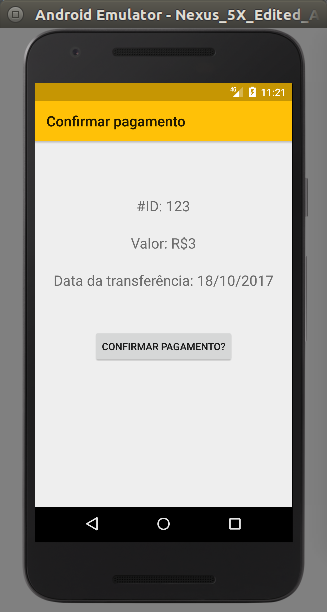
\includegraphics[scale=0.5]{int:confirm}
		\caption{Interface de confirma\c{c}\~ao com\\\hspace{\textwidth}os dados preenchidos na \ref{int:pay_img}}
		\label{int:confirm}
	\end{subfigure}
	\caption{Confirma\c{c}\~ao dos dados de uma transa\c{c}\~ao}
	\label{pay_composite}
\end{figure}

Ap\'os o desenvolvimento desses dois aplicativos considerei ter adquirido um conhecimento suficiente para prosseguir e dar início ao desenvolvimento da interface do aplicativo alvo deste trabalho. \'E claro que passei por um n\'umero pequeno de componentes que o \textit{Android} possui, existem diversos outros \textit{Fragments} que executam diferentes tarefas de diferentes formas visuais, além de muitos outros componentes que at\'e o momento da finaliza\c{c}\~ao desse aplicativo n\~ao vi como necess\'arios para este desenvolvimento em espec\'ifico.

\subsection{Desenvolvimento das interfaces do aplicativo} \label{dev}

Finalizada a etapa de aprendizado em \textit{Android}, dei in\'icio ao segundo objetivo do trabalho que consistia em desenhar as interfaces do aplicativo de micropagamentos operando sobre uma base de servi\c{c}os funcional. O primeiro passo foi a familiariza\c{c}\~ao com a plataforma, entender o fluxo de execu\c{c}\~ao, os triggers, os listeners, estudar literalmente a plataforma inteira, nessa parte contei com a colabora\c{c}\~ao do \textbf{Henrique Leme}, desenvolvedor da plataforma, com o aux\'ilio dele essa parte foi facilitada permitindo que a assimila\c{c}\~ao do conteúdo fosse mais flu\'ida.

Passada essa parte foi definido que o desenvolvimento seria principalmente no diret\'orio \textit{res}, na estrutura de um projeto \textit{Android}, nesse diret\'orio ficam todos os arquivos relacionados a parte visual do aplicativo, as interfaces, os \'icones, as imagens, defini\c{c}\~oes de estilos, \textit{Strings}, etc. Tamb\'em foi preciso em alguns pontos fazer modifica\c{c}\~oes no \textit{MainActivity}, j\'a que algumas interfaces precisaram ser mapeadas e algumas a\c{c}\~oes foram reescritas para atender o novo formato no \textit{layout}.

Uma mudan\c{c}a substancial no desenvolvimento dessas interfaces foi o uso do \textit{Relative Layout} ao inv\'es do \textit{Constraint Layout} que foi usado nos dois aplicativos descritos na sub-se\c{c}\~ao \ref{learn}. Durante a execu\c{c}\~ao dos dois aplicativos anteriores esse detalhe passou desapercebido durante o desenvolvimento, o que ocasionou um certo volume de trabalho para estabelecer a posi\c{c}\~ao de cada componente na tela. A vantagem no uso do \textit{Relative Layout} \'e poder declarar a posi\c{c}\~ao dos componentes de acordo com seus parentes ou seus irm\~aos, ele d\'a um maior controle sobre os itens no \textit{layout}. Por exemplo, temos uma \textit{view} que define uma \'area retangular na interface, e dentro dessa \'area precisam estar 3 outros componentes, vamos dizer bot\~oes, e esses 3 componentes precisam estar alinhados à direita da \'area. Com o \textit{Relative Layout} declaramos a \'area, o primeiro bot\~ao alinhado a direita da \'area, e cada um dos bot\~oes subsequentes um abaixo do outro, o c\'odigo para esta ilustrado na \textit{listing} \ref{relative}.
\begin{lstlisting}[language=XML, caption=\textit{Exemplo de uso de um \textit{RelativeLayout}}, captionpos=b, breaklines=true, label=relative]
<RelativeLayout xmlns:android="http://schemas.android.com/apk/res/android"
	android:layout_width="match_parent"
	android:layout_height="match_parent"
	android:paddingLeft="16dp"
	android:paddingRight="16dp">
	<Button
		android:id = "@+id/box1"
		android:layout_width="wrap_content"
		android:layout_height="wrap_content"
		android:layout_alignParentLeft="true"
		android:text="button1" />
	<Button
		android:id = "@+id/box2"
		android:layout_width="wrap_content"
		android:layout_height="wrap_content"
		android:layout_below="@id/box1"
		android:layout_alignParentLeft="true"
		android:text="button2" />
	<Button
		android:id = "@+id/box3"
		android:layout_width="wrap_content"
		android:layout_height="wrap_content"
		android:layout_below="@id/box2"
		android:layout_alignParentLeft="true"
		android:text="button3" />
</RelativeLayout>
\end{lstlisting}
A exce\c{c}\~ao do aprendizado do \textit{Relative Layout} n\~ao houve grandes dificuldades no desenvolvimento das interfaces visto que a maior parte deles foi escrita usando bot\~oes e campos textos para carregar as informa\c{c}\~oes. De componentes e t\'ecnincas n\~ao vistos na etapa de arendizado foram utilizados o \textit{Spinner}, e a declara\c{c}\~ao de todas as \textit{Strings} em um arquivo \textit{XML} \`a parte.

O \textit{Spinner} \'e um componente que permite selecionar um valor de uma lista de op\c{c}\~oes poss\'iveis, quando n\~ao selecionado ele assume um valor padr\~ao pr\'e-definido, quando selecionado ele exibe em uma lista todos os valores dispon\'iveis, quando um valor \'e selecionado ele fica exibido onde previamente estava o valor padr\~ao. No aplicativo essa lista \'e obtida de outros dispostivos que foram pareados por bluetooth com o do usu\'ario.
Na interface \'e necess\'ario apenas adicionar o elemento \textit{\textless{Spinner}\textgreater} no c\'odigo, com suas respectivas propriedades, e na parte do controlador \'e preciso sobreescrever os m\'etodos que definem o que deve ser feito quando o usu\'ario seleciona um item e o que deve ser feito se nada for selecionado.

A segunda mudan\c{c}a foi o uso de um arquivo \textit{XML} para armazenar todas as \textit{Strings} usadas no aplicativo. As vantagens dessa abordagem, ao contr\'ario de escrever manualmente todas elas diretamente, \'e a flexibilidade e a reusabilidade.

Flexibilidade pois tendo o arquivo como base \'e poss\'ivel traduzir ele para outros idiomas, como o id das \textit{strings} permanece o mesmo, as mesmas j\'a est\~ao referenciadas no c\'odigo e v\~ao exibir o valor definido. Isto \'e útil para se localizar o aplicativo para outros pa\'ises que usam uma linguagem diferente da que se foi desenvolvido o aplicativo inicialmente.

Reusabilidade porque elas s\~ao apenas referenciadas no c\'odigo, qualquer mudan\c{c}a que for feita em um dos valores \'e replicada por todo o aplicativo poupando o trabalho de precisar reescrever todas as ocorrências e correr o risco de esquecer alguma, al\'em da possibilidade de usar uma mesma palavra em diversos elementos do aplicativo sem a necessidade de escrever o mesmo repetidas vezes.
\section{Considera\c{c}\~oes Finais}
No in\'icio do projeto foram definidos dois objetivos para este trabalho, aprender o desenvolvimento para \textit{Android} e aplicar o conhecimento adquirido para produzir as interfaces de um aplicativo. Sendo o primeiro pr\'e-requisito obrigat\'orio para a execu\c{c}\~ao do segundo, \'e mais prudente discorrer sobre ele de in\'icio.

O desenvolvimento para \textit{Android} conta com uma boa base de conhecimento e materiais no pr\'oprio site tanto de t\'opicos b\'asicos, como por exemplo um guia de configura\c{c}\~ao do ambiente, at\'e mais avan\c{c}ados, como a documenta\c{c}\~ao de cada componente da plataforma, que pode ser considerado suficiente para qualquer um que tenha interesse em aprender a desenvolver aplicativos para \textit{Android} consiga fazer o mesmo. É bem verdade que em alguns assuntos a documenta\c{c}\~ao \'e um pouco confusa ou peca pela falta de exemplos mais concretos de implementa\c{c}\~ao, mas, como dito na se\c{c}\~ao \ref{revisao}, f\'oruns e sites na internet existem em grandes quantidades com outras pessoas com dúvidas similares ou aproximadamente iguais, e a maoria com solu\c{c}\~oes para tais empecilhos. Um problema recorrente nisso \'e talvez a falta de uma solu\c{c}\~ao única, para um mesmo problema podem existir n solu\c{c}\~oes diferentes, o que exige muita an\'alise e testes para descobrir quais, ou qual, \'e a mais adequada para o problema encontrado.

Isso era comum de se encontrar tanto para problemas de interfaces, como por exemplo como fazer uma imagem caber dentro de um bot\~ao, como para problemas de \textit{back-end}, como por exemplo qual a melhor abordagem para implementar \textit{Fragments} em elementos do \textit{layout}.

Apesar disso considero que a plataforma apresenta uma dificuldade m\'edia de aprendizado, alguns elementos s\~ao de f\'acil assimila\c{c}\~ao ao passo que alguns exigem um pouco mais de estudo e pesquisa para se entender o que precisa ser feito para atingir o resultado esperado. As interfaces s\~ao mais f\'aceis de compreender como se desenvolver do que como prograrmar os controles que gerenciam o funcionamento da aplica\c{c}\~ao.

Considero que \'e poss\'ivel sim aprender sozinho o suficiente para criar um aplicativo simples usando as informa\c{c}\~oes que se encontra nas documenta\c{c}oes oficiais e nas literaturas sobre o assunto, mas para projetos de larga escala acredito ser dif\'icil de conseguir o resultado desejado apenas com esses recursos.

Quanto ao segundo objetivo, mantenho o que foi dissertado na sub-se\c{c}\~ao \ref{dev} em rela\c{c}\~ao ao desenvolvimento das mesmas, uma das premissas era que as interfaces do aplicativo fossem de f\'acil usablidade, com isso em foco, considerei mais prudente n\~ao precisar fazer nada que fosse apenas visualmente mais atraente mas de d\'ificil asssimi\c{c}\~ao e foquei em pensar na solu\c{c}\~ao que fosse de mais f\'acil compreens\~ao qual a\c{c}\~ao deveria ser tomada em cada umas das interfaces. É claro que sem a primeira parte do aprendizado esta etapa teria possu\'ido uma dificuldade exrememamente maior de ser realizada, j\'a que ao mesmo tempo seria necess\'ario entender o funcionamento e desenvolver os componentes nas interfaces.

Uma futura possibilidade que poderia ser considerada como uma extens\~ao desse trabalho seria tentar adaptar o aplicativo usando a linguagem \textit{Kotlin}. Recentemente os respons\'aveis pelo \textit{Android} anunciaram que a plataforma passaria a oferecer suporte para a linguagem \cite{kotlin:and_adopt}. O site da \textit{Wired} publicou um artigo em que diz que a linguagem \'e a nova tendência no Vale do Sil\'icio e que passaremos a ver cada vez mais aplicativos desenvolvidos nela \cite{kotlin:wired}.

Para este trabalho em espec\'ifico o \textit{Kotlin} entrou mais como uma curiosidade, j\'a que o foco dele era desenvolvimento em \textit{Android} puro, por\'em foi algo que despertou grande curiosidade em explorar essa nova linguagem e medir a diferen\c{c}a do tempo de aprendizagem e implementa\c{c}\~ao de um aplicativo usando cada uma das linguagens.
%Final do doc
\newpage
\section*{Refer\^encias Bibliogr\'aficas}
\addcontentsline{toc}{section}{Refer\^encias Bibliogr\'aficas}
\renewcommand\refname{}
\bibliography{helper}
\bibliographystyle{unsrt}
\newpage
\appendix
\renewcommand\thefigure{\thesection.\arabic{figure}}
\setcounter{figure}{0} 
\begin{appendices}
	\section{Fluxo do aplicativo}
	Aqui ser\'a descrito o funcionamento do aplicativo
	
	\begin{figure}[h]
		\centering
		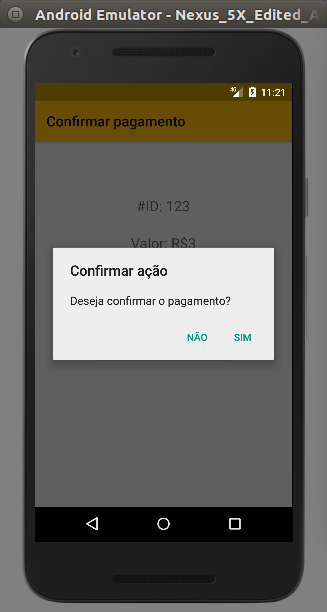
\includegraphics[scale=0.2]{int:confirm_confirm}
		\caption{sample}
		\label{sample}
	\end{figure}
\end{appendices}
\end{document}